\documentclass[A4,svgnames,9pt,aspectratio=169]{beamer}
%% document options:
%% - aspectratio = { 43, 169, 1610 }
%% - utf8
%%

%%
%% insert list of packages
%%
\usepackage{pgfplots}
\pgfplotsset{compat=1.17}

%% \usepackage[english,french]{babel}

\hypersetup{
   allcolors=rouge_inria,
   pdfauthor   = {firstname lastname},
   pdftitle    = {\@title},
   pdfsubject  = {Resum\'{e} of everything},
   pdfkeywords = {firstname~lastname, curriculum vit\ae{}}
}

\usepackage[doi=false,isbn=false,url=false,natbib=true,style=numeric,backend=bibtex,useprefix=true]{biblatex}
\addbibresource{frames/biblio.bib}
\usepackage{tikz}
\usetikzlibrary{shapes, arrows, positioning, fit}

%%%%%%%%%%%%%%%%%%%%%%%%%%%%%%%%%%%%%%%%%%%%%%%%%%%%%%%
%%
%%%%%%%%%%%%%%%%%%%%%%%%%%%%%%%%%%%%%%%%%%%%%%%%%%%%%%%

\title[titrecourt]{Scalable Hyperparameter Optimization\\ for LLM
Fine-Tuning}
\subtitle{Bayesian and Partition-based optimization}
\date[20/01/2025]{date long}
\author[A. et al.]{N. Davouse}

\usetheme{inria}
\usepackage{multirow}
\usepackage{booktabs}
\usepackage{amsmath}
\usepackage{algorithm}
\usepackage{algorithmic}


\begin{document}

%%%%%%%%%%%%%%%%%%%%%%%%%%%%%%%%%%%%%%%%%%%%%%%%%%%%%%%
%%
%%%%%%%%%%%%%%%%%%%%%%%%%%%%%%%%%%%%%%%%%%%%%%%%%%%%%%%

\frame{\titlepage}

%%%%%%%%%%%%%%%%%%%%%%%%%%%%%%%%%%%%%%%%%%%%%%%%%%%%%%%

% Le titre des planches de sommaire est \contentsname, sa valeur
% est fixée ici à "Sommaire" par défaut.
\renewcommand{\contentsname}{Summary}

% Si le package babel est utilisé la valeur
% prend celle par défaut de la langue sélectionnée.
% Pour imposer une valeur, y compris lors de l'utilisation de
% babel, faire attention à redéfinir cette variable _après_
% un \selectlanguage{}

% \selectlanguage{french}
% \selectlanguage{english}

\frame{\tocpage}

%%%%%%%%%%%%%%%%%%%%%%%%%%%%%%%%%%%%%%%%%%%%%%%%%%%%%%%
\section{Introduction}
\frame{\sectionpage}
%---------------------------------- Large Language Models -------------------------------
\begin{frame}{Large Language Models}
\begin{columns}
      
    \begin{column}[t]{0.4\textwidth}
    \begin{block}{Summary}
    
        \begin{itemize}
            \item State-of-the-art of Natural Language Processing (NLP) problems
            \item Architecture : Transformers\cite{NIPS2017_3f5ee243} block, mixed with classical layers (MLP, Conv)
            \item Huge size : Billions of parameters (1B to 405B for Llama 3)
            \item 2 phases of training : pre-training and \textbf{fine-tuning}
        \end{itemize}
            

    \end{block}
    \end{column}
        
    \begin{column}[t]{0.55\textwidth}
    \begin{block}{Self Attention }

        \begin{figure}
            \centering
            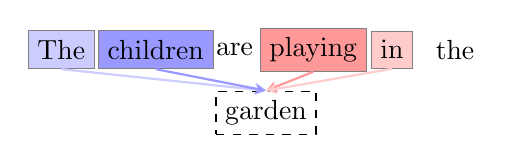
\begin{tikzpicture}[node distance=0.8cm]

% Define block styles
\tikzstyle{model} = [rectangle,rounded corners, minimum width=2cm, minimum height=1cm, text centered, draw=black, fill=blue!30]
\tikzstyle{arrow} = [thick,->,>=stealth]

% Define nodes
\node (the) [fill=blue!20,rectangle,draw=black!50] {The};
\node (children) [right of = the,fill=blue!40,rectangle,draw=black!50,xshift=0.4cm] {children};
\node (are) [right of = children,xshift=0.2cm] {are};
\node (playing) [right of = are,fill=red!40,rectangle,draw=black!50,xshift=0.2cm] {playing};
\node (in) [right of = playing,fill=red!20,rectangle,draw=black!50,xshift=0.2cm] {in};
\node (the2) [right of = in] {the};

\node (garden) [below of = are, xshift=0.4cm,rectangle,dashed,draw=black] {garden};

% Draw arrows
\draw [arrow,draw=blue!20] (the.south) -- (garden.north);
\draw [arrow,draw=blue!40] (children.south) -- (garden.north);
\draw [arrow,draw=red!40] (playing.south) -- (garden.north);
\draw [arrow,draw=red!20] (in.south) -- (garden.north);

% Add a rectangle around the last four nodes
\end{tikzpicture}
            \caption{Self Attention mecanism illustration}
        \end{figure}
    
        Self attention is the key of LLM, used to compute the context of each token.
    \end{block}  
    \end{column}
         
\end{columns}
\end{frame}

%---------------------------------- Fine-tuning Workflow -------------------------------

\begin{frame}{Fine-Tuning}
    Fine-tuning is used to correct behavior or add in-domain data to a model, with limited ressources. 


    \begin{figure}
        \centering
        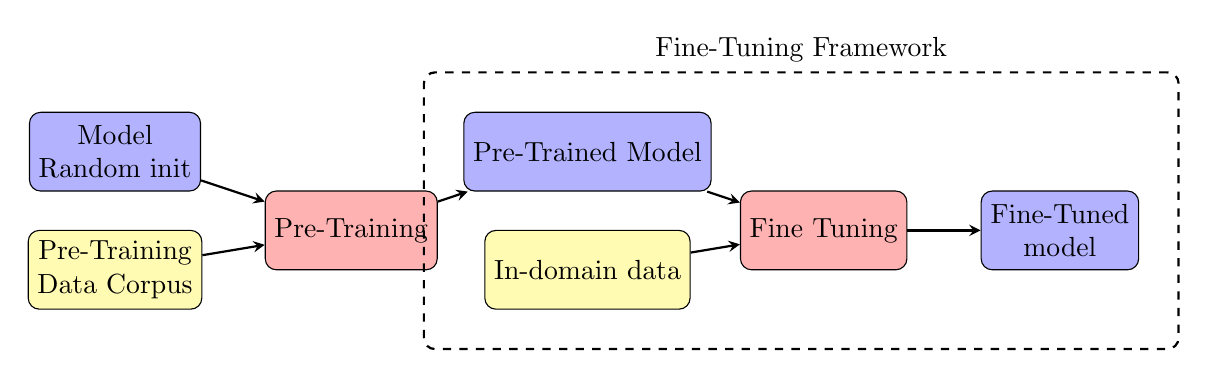
\begin{tikzpicture}[node distance=1.5cm]

% Define block styles
\tikzstyle{model} = [rectangle,rounded corners, minimum width=2cm, minimum height=1cm, text centered, draw=black, fill=blue!30]
\tikzstyle{data} = [rectangle, rounded corners, minimum width=2cm, minimum height=1cm,text centered, draw=black, fill=yellow!30]
\tikzstyle{action} = [rectangle, rounded corners, minimum width=2cm, minimum height=1cm,text centered, draw=black, fill=red!30]
\tikzstyle{arrow} = [thick,->,>=stealth]

% Define nodes
\node (model1) [model,align=center] {Model\\Random init};
\node (data1) [data, below of=model1,align=center]{Pre-Training \\ Data Corpus} ;
\node (pre-train)[action, right of=model1, xshift=1.5cm,yshift=-1cm]{Pre-Training};
\node (model2) [model, right of=pre-train, xshift = 1.5cm, yshift=1cm ]{Pre-Trained Model};
\node (data2) [data, below of= model2]{In-domain data};
\node (fine-tuning)[action, right of = model2, xshift = 1.5cm,yshift=-1cm]{Fine Tuning};
\node (model3) [model, right of=fine-tuning, xshift = 1.5cm,align=center ]{Fine-Tuned \\ model};


% Draw arrows
\draw [arrow] (data1) -- (pre-train);
\draw [arrow] (model1) -- (pre-train);
\draw [arrow] (pre-train) -- (model2);
\draw [arrow] (model2) -- (fine-tuning);
\draw [arrow] (data2) -- (fine-tuning);
\draw [arrow] (fine-tuning) -- (model3);

% Add a rectangle around the last four nodes
\node[draw, thick, dashed, rounded corners, fit=(model2) (fine-tuning) (model3) (data2), inner sep=0.5cm, label=above:{Fine-Tuning Framework}] {};
\end{tikzpicture}
        \caption{Pre-training and Fine-tuning generic workflow}
    \end{figure}  
        

    
\end{frame}

%---------------------------------- Fine Tuning Frame -------------------------------
\begin{frame}{Parameters Efficient Fine-Tuning (PEFT)}
    Set of methods aims to reduce the computation cost of fine-tuning. 2 approachs : \textit{Additive} and \textbf{reparametrization}.
    


    
    \begin{columns}  
  
        \begin{column}[t]{0.45\textwidth}
        \begin{block}{Reparametrization}
            Use lower-cost proxy as trainable weights, and merge at the end. Most famous method : LoRA \cite{hu2021loralowrankadaptationlarge}. These methods are hyperparameter-dependent.
        \end{block}
        \end{column}
    
        \begin{column}[t]{0.45\textwidth}
        \begin{block}{Addivitive}
            Add part of the model, often linear layer, to train these.  One con is to add inference to generation.
            
        \end{block}
        \end{column}
      
    \end{columns}

\end{frame}



%---------------------------------- LoRA -------------------------------
\begin{frame}{Low Rank Adaptation (LoRA)}
    \begin{block}{Principle}
        Merging Fine-tuning layers with pre-trained ones can be written as $W = W_0 + \Delta W$, with $W_0$ the pre-trained weights and $\Delta W$ the fine-tuned ones.         
    \end{block}

    \begin{columns}
        \begin{column}[t]{0.45\textwidth}
        \begin{figure}
            \centering
            %\includegraphics[width=0.5\linewidth]{imgs/lora.png}
            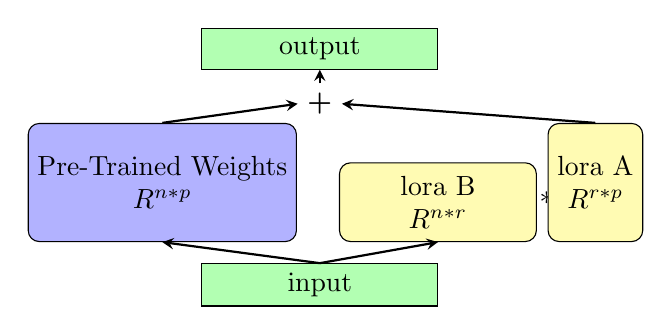
\begin{tikzpicture}[node distance=1.5cm]
% Define block styles
\tikzstyle{weights} = [rectangle,rounded corners, minimum width=2.5cm, minimum height=1.5cm, text centered, draw=black, fill=blue!30]
\tikzstyle{lora_a} = [rectangle,rounded corners, minimum width=1cm, minimum height=1.5cm, text centered, draw=black, fill=yellow!30]
\tikzstyle{lora_b} = [rectangle,rounded corners, minimum width=2.5cm, minimum height=1cm, text centered, draw=black, fill=yellow!30]
\tikzstyle{vector} = [rectangle, minimum width=3cm, minimum height=0.5cm, text centered, draw=black, fill=green!30]
\tikzstyle{arrow} = [thick,->,>=stealth]

% Define nodes
\node (weights) [weights, align=center]{Pre-Trained Weights \\ $\mathbb{R}^{n*p}$};
\node (lora_B) [lora_b, right of=weights,xshift=2cm,yshift=-0.25cm, align=center]{lora B\\ $\mathbb{R}^{n*r}$};
\node (mul) [right of = lora_B,xshift=-0.12cm]{*};
\node (lora_A) [lora_a, right of=lora_B,xshift=0.5cm,yshift=0.25cm, align=center]{lora A\\$\mathbb{R}^{r*p}$};
\node (input) [vector,below of = weights, xshift = 2cm,yshift=+0.2cm]{input};
\node (plus) [above of = weights, xshift = 2cm,yshift=-0.5cm]{\textbf{+}};
\node (output) [vector,above of = plus,yshift=-0.8cm]{output};




% Draw arrows
\draw [arrow] (input.north) -- (weights.south);
\draw [arrow] (input.north) -- (lora_B.south);
\draw [arrow] (weights.north) -- (plus.west);
\draw [arrow] (lora_A.north) -- (plus.east);
\draw [arrow] (plus) -- (output);


\end{tikzpicture}
            \caption{LoRA Decomposition}
        \end{figure}
            
        \end{column}
        
        \begin{column}[t]{0.3\textwidth}
            \begin{block}{LoRA hyperparameters}
            \begin{itemize}
                \item rank : the common dimension between $A$ and $B$.
                \item alpha : apply a weighting between fine-tuning and pre-trained weights
            \end{itemize}
                
            \end{block}
            
        \end{column}
    \end{columns}
    
\end{frame}

%%%%%%%%%%%%%%%%%%%%%%%%%%%%%%%%%%%%%%%%%%%%%%%%%%%%%%%

%%%%%%%%%%%%%%%%%%%%%%%%%%%%%%%%%%%%%%%%%%%%%%%%%%%%%%%
\section{Review of Related Works}
\frame{\sectionpage}
%---------------------------------- Prompt Engineering -------------------------------
\begin{frame}{Prompt Engineering}
    Prompt : process of interacting with an artificial intelligence (AI) system by providing specific instructions or queries to achieve a desired outcome. 

    Example with article \cite{guo_connecting_2024}, when a second LLM is used to modify the prompt.

    \begin{columns}
        
        \begin{column}[t]{0.45\textwidth}
            \begin{block}{Pros}
                Don't need to deal with architecture, weights : 
                act like the LLM is a generating blackbox
                
            \end{block}

        \end{column}

        \begin{column}[t]{0.45\textwidth}
            \begin{block}{Cons}
                Low impact, locate this work as the end-user, not so much usable
                
            \end{block}

        \end{column}

    \end{columns}

    
\end{frame}

%---------------------------------- LLM to Optimization -------------------------------
\begin{frame}{LLM applied to Optimization}
    Multiples articles show the use of LLM to develop or code optimization algorithms, in particular Evolutionnary Algorithm. One intersting impact is to popularize the development of optimization algorithm.

    \begin{columns}
        
        \begin{column}[t]{0.45\textwidth}
            \begin{block}{Pros}
                Extend the fields of Meta-Heuristics, with new kinds of operators. 
                
            \end{block}

        \end{column}

        \begin{column}[t]{0.45\textwidth}
            \begin{block}{Cons}
                Low impact, don't achieve remarkable performance. 
            \end{block}

        \end{column}

    \end{columns}

    
\end{frame}

%---------------------------------- Auto DNN -------------------------------
\begin{frame}{Auto DNN}
    \begin{block}{Sub-domains}
        \begin{itemize}
            \item \textbf{HyperParameter Optimization(HPO) : Automaticaly define best hyper-parameters, from training to inference} 
            \item Neural Architecture Search(NAS) : Define the best architecture, from scratch or from pruning an existing one
        \end{itemize}
        
    \end{block}


    \begin{block}{Metrics}
        \begin{itemize}
            \item Performance metrics : Accuracy, Latency
            \item Ressource metrics : inference time, memory usage, energy consumption
        \end{itemize}
        
    \end{block}
    
\end{frame}

%---------------------------------- Review Summary -------------------------------
\begin{frame}{Summary}
    \begin{figure}
        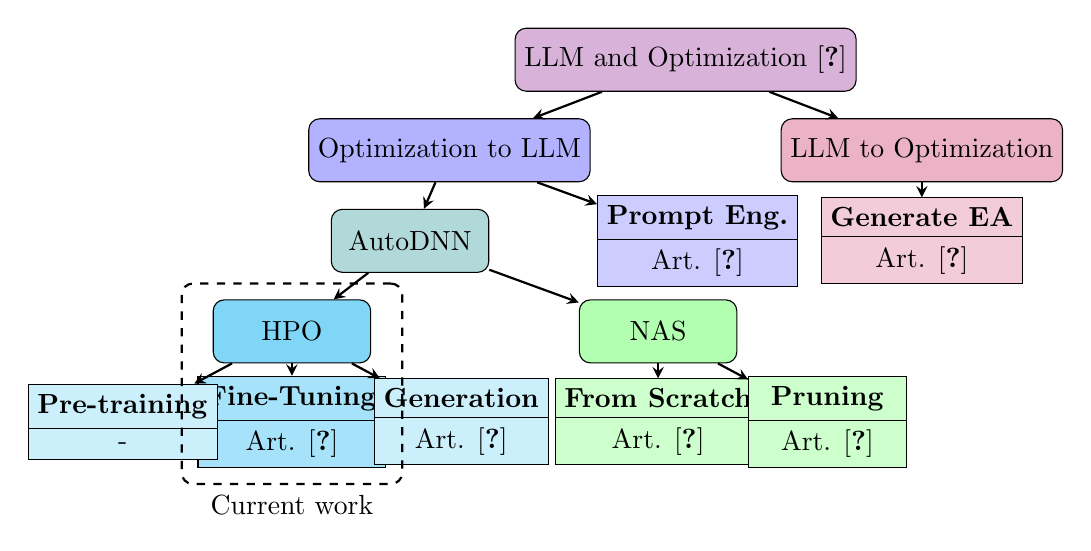
\begin{tikzpicture}[node distance = 1.15cm]

\tikzstyle{field} = [rectangle,rounded corners, minimum width=2cm, minimum height=0.8cm, text centered, draw=black]
\tikzstyle{art} = [rectangle split, rectangle split parts = 2, minimum width=2cm, minimum height=0.8cm, text centered, draw=black, fill=blue!30]
\tikzstyle{arrow} = [thick, ->, >=stealth]


% base
\node (base)[field, fill = violet!30]{LLM and Optimization \cite{wu_evolutionary_2024}};

% lvl 1
\node (opt_llm)[field, below of = base, xshift = -3cm, fill = blue!30]{Optimization to LLM};

\node (llm_opt)[field, below of = base, xshift = 3cm, fill = purple!30]{LLM to Optimization};

% lvl 2
\node (autodnn)[field, below of = opt_llm, xshift = -0.5cm, fill=teal!30]{AutoDNN};
\node(prompt)[art,right of = autodnn, xshift = 2.5cm, fill = blue!20]{
    \textbf{Prompt Eng.}
    \nodepart{second} Art. \cite{guo_connecting_2024}
};
\node (gen_ea)[art, below of = llm_opt, fill = purple!20]{
    \textbf{Generate EA}
    \nodepart{second} Art. \cite{liu_large_2024}
};

% lvl 3
\node (hpo)[field, below of = autodnn, xshift = -1.5cm, fill = cyan!50]{HPO};
\node (nas)[field, right of = hpo, xshift = 3.5cm, fill = green!30]{NAS};

% lvl4 hpo

\node (hpo_ft)[art, below of = hpo, fill = cyan!35]{
    \textbf{Fine-Tuning}
    \nodepart{second} Art. \cite{tribes_hyperparameter_2024}
};
\node (hpo_pt)[art, left of = hpo_ft, xshift = -1cm, fill = cyan!20]{
    \textbf{Pre-training}
    \nodepart{second} -
};
\node (hpo_gen)[art, right of = hpo_ft,xshift = 1cm, fill = cyan!20]{
    \textbf{Generation}
    \nodepart{second} Art. \cite{wang_cost-effective_2023}
};
% lvl4 nas
\node (nas_scratch)[art, below of = nas, fill = green!20]{
    \textbf{From Scratch}
    \nodepart{second} Art. \cite{gao_autobert-zero_2022}
};
\node (nas_pruning)[art, right of = nas_scratch,xshift = 1cm, fill = green!20]{
    \textbf{Pruning}
    \nodepart{second} Art. \cite{klein_structural_2023}
};

% arrows
\draw[arrow] (base) -- (opt_llm);
\draw[arrow] (base) -- (llm_opt);

\draw[arrow] (opt_llm) -- (autodnn);
\draw[arrow] (opt_llm) -- (prompt);
\draw[arrow] (llm_opt) -- (gen_ea);

\draw[arrow] (autodnn) -- (hpo);
\draw[arrow] (autodnn) -- (nas);

\draw[arrow] (hpo) -- (hpo_pt);
\draw[arrow] (hpo) -- (hpo_ft);
\draw[arrow] (hpo) -- (hpo_gen);

\draw[arrow] (nas) -- (nas_scratch);
\draw[arrow] (nas) -- (nas_pruning);

% fitting box
\node (current)[draw,thick, dashed, rounded corners, 
    fit = (hpo)(hpo_ft), inner sep = 0.2cm,
    label = below :{Current work}]{};

\end{tikzpicture}
        \caption{Summary of links between LLM and Optimization}
    \end{figure}
    
    
\end{frame}
%%%%%%%%%%%%%%%%%%%%%%%%%%%%%%%%%%%%%%%%%%%%%%%%%%%%%%%

%%%%%%%%%%%%%%%%%%%%%%%%%%%%%%%%%%%%%%%%%%%%%%%%%%%%%%%
\section{Problem Definition}
\frame{\sectionpage}
%---------------------------------- Problem definition -------------------------------
\begin{frame}{Problem Definition}
    This problem can be characterized the optimization of an \large\textbf{expensive, mixed-variable, noisy, blackbox} function.

    \begin{columns}
    
        \begin{column}[t]{0.5\textwidth}
        \begin{block}{Problem Formulation}
            The HPO problem can be defined as 
            \begin{equation}
               \eta^* \in \arg\min_{\eta \in \mathcal{H}} \mathcal{F}(\eta) 
            \end{equation}

        \end{block}

        \begin{block}{Search Space $\mathcal{H}$}
            $\mathcal{H}$ is the set of all values the solution tuple $\eta$ can take. This stage includes method to handle the mixed-variables aspect of the problems.   
        \end{block}
        \end{column}
        
        \begin{column}[t]{0.5\textwidth}

    
        \begin{block}{Search Strategy}
            With $\eta_i$ all the tested solutions, the search strategy is the method used to define the next solution $\eta_{next}$ to evaluate. 
        \end{block}

        \begin{block}{Perfomance Evaluation Strategy}
            $\mathcal{F}$ represent the objective function, how the function is implemented. Also includes method like multi-fidelity that affect the fidelity of the evaluation.
        \end{block}

        \end{column}
         
  \end{columns}
\end{frame}


%------------------------------------ Search Space ---------------------------
\begin{frame}{Search Space}

    The search space is composed of variables of different type.

    \begin{block}{Hyper-parameters}
    
        \begin{table}[h!]
            \centering
            \begin{tabular}{|c|c|c|c|}
                \hline
                \multirow{2}{*}{\textbf{Hyper-parameter}} & \multicolumn{2}{|c|}{\textbf{Optimization range}} & \multirow{2}{*}{\textbf{Conversion}} \\
                \cline{2-3}
                 & \textbf{Lower Bound} & \textbf{Upper Bound} &  \\
                \hline
                \textbf{Learning Rate} & $-10$ & $-1$ & $f(x) = 10^{x}$ \\
                \hline
                \textbf{LoRA Rank} & 2 & 512 & $f(x) = \text{round}(x)$ \\
                \hline
                \textbf{LoRA scale ($\alpha$)} & 1 & 64 & $f(x) = \text{round}(x)$ \\
                \hline
                \textbf{LoRA Dropout} & 0 & 0.5 & $f(x) = x$ \\
                \hline
                \textbf{Weight Decay} & $-5$ & $-1$ & $f(x) = 10^{x}$  \\
                \hline
            \end{tabular}
            \caption{Summary of Hyperparameter Search Space}
            \label{tab:hyperparam_table}
        \end{table}
        
    \end{block}
    
    Conversion and naming convention is taken from LitGPT framework.
\end{frame}


%---------------------------------- Search Strategy  -------------------------------
\begin{frame}{Search Strategy}
    The search strategy of an optimization problem can be seen as a balance between the exploration, i.e. going to unexplored regions, and exploitation, i.e. going close to promising areas. Here are the fields of optimization to tackle HPO problems. Standard optimization fields : 
    \begin{itemize}
        \item sampling/exploratory : Grid Search, Random Search, Latin Hypercube Sampling \\ \quad no exploitation, give a lower bound
        \item Bayesian Optimization : use surrogate to approximate the objective function, and optimize it. \\ \quad weak parallel ability, strong exploitation
        \item Partition-Based Optimization : FDA, SOO, DiRect \\ \quad innate parallel ability, slow convergence
    \end{itemize}

\end{frame}
%---------------------------------- Performance Evaluation Strategy -------------------------------

\begin{frame}{Performance Evaluation Strategy}
    \begin{block}{Evaluation context}
    In this part, there are many options, like the number of epochs (if not an hyperparameters), the precision of the model, the datasets of training or evaluation. 
        
    \end{block}
    \begin{block}{Objective function}
        For this problem, there are 2 ways to evaluate a solution : 
        \begin{itemize}
            \item Loss (validation or testing) : the loss is computed through the training, and we can keep a small part of the datasets unused to use it the evaluate the model. Cons : dataset dependant, difficult to put in global context
            \item \textbf{Benchmark dataset (GLUE\cite{wang2018glue}, MMLU\cite{hendrycks2021mmlu})} : the accuracy on a literature benchmark dataset can be used to evaluate the training. It's interesting, since it's a good measure of generalization, since the model has not read this type of questions. Warning : the benchmark used during the optimization can't be used as a final testing. 
        \end{itemize}

        Multi-fidelity approaches can be used to reduce the cost of evaluation in earlier steps. Algorithms like Bayesian Optimization and HyperBand (BOHB\cite{DBLP:journals/corr/abs-1807-01774}) achieve cost-efficient optimization by reducing the part of the datasets in early stages.
    \end{block}
    
\end{frame}
%%%%%%%%%%%%%%%%%%%%%%%%%%%%%%%%%%%%%%%%%%%%%%%%%%%%%%%

%%%%%%%%%%%%%%%%%%%%%%%%%%%%%%%%%%%%%%%%%%%%%%%%%%%%%%%
\section{Methodology}
\frame{\sectionpage}
%---------------------------------- Optimization frame -------------------------------
\begin{frame}{Global HPO workflow}
            \begin{figure}
                \centering
                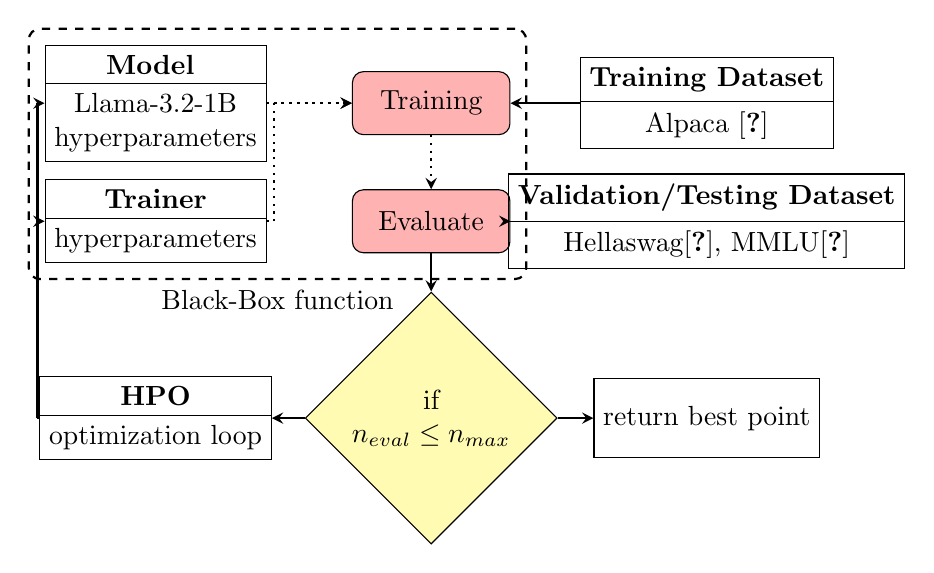
\begin{tikzpicture}[node distance=1.5cm]

    % Define block styles
    \tikzstyle{class}=[rectangle split,rectangle split parts=2,draw,text centered]
    \tikzstyle{action} = [rectangle, rounded corners, minimum width=2cm, minimum height=0.8cm,text centered, draw=black, fill=red!30]
    \tikzstyle{decision} = [diamond,text centered, draw=black, fill=yellow!30]
    \tikzstyle{final} = [rectangle, minimum width=2cm, minimum height=1cm,text centered, draw=black]
    
    % Define arrow styles
    \tikzstyle{tarrow} = [thick,->,>=stealth]
    \tikzstyle{larrow} = [thick,dotted,->,>=stealth]
    \tikzstyle{coin} = [thick]
    \tikzstyle{light} = [thick,dotted]
    
    
    % Define nodes
    
    % black box function
    \node (model) [class, align=center]
        {
            \textbf{Model }
            \nodepart{second} Llama-3.2-1B \\ hyperparameters };  
    
    \node (trainer) [class, below of=model]
        {
            \textbf{Trainer}
            \nodepart{second} hyperparameters};
    
    \node (training)[action,right of = model,xshift=2cm]{Training};
    \node (evaluate)[action,below of = training]{Evaluate};
    
    \node(bbfunction)[draw, thick, dashed, rounded corners, fit=(model) (trainer) (training) (evaluate), inner sep=0.2cm, label=below:{Black-Box function}] {};
    
    
    %datasets
    \node (train_data) [class, right of=training,xshift=2cm]
        {
            \textbf{Training Dataset}
            \nodepart{second} Alpaca \cite{hashimoto_stanford_2024}};
    
    \node (val_data) [class, right of=evaluate,xshift=2cm]
        {
            \textbf{Validation/Testing Dataset}
            \nodepart{second} Hellaswag\cite{zellers_hellaswag_2019}, MMLU\cite{hendrycks_measuring_2021}};
    
    % decision
    \node (decision)[decision,below of = evaluate,yshift=-1cm,align=center]{if \\ $n_{eval} \leq n_{max}$ };
    
    \node (final)[final,right of = decision,xshift=2cm]{return best point};
    
    % HPO
    \node (hpo) [class, below of=trainer,yshift=-1cm]
        {
            \textbf{HPO}
            \nodepart{second} optimization loop};
    
    
    % functionnal node
    \node (trainerright) [right of=trainer]{};
    \node (modelright) [right of=model]{};
    \node (hpoleft) [left of = hpo]{};
    \node (modelleft) [left of = model]{};
    \node (trainerleft) [left of = trainer]{};
    
    
    % arrow inside bb function
    \draw [larrow] (model) -- (training);
    \draw [light] (trainer) -- (trainerright.center);
    \draw [light] (trainerright.center) -- (modelright.center);
    \draw [larrow] (modelright.center) -- (training);
    \draw [larrow] (training) -- (evaluate);
    
    % arrows outside bb function
    \draw [tarrow] (train_data) -- (training);
    \draw [tarrow] (val_data) -- (evaluate);
    \draw [tarrow] (evaluate) -- (decision);
    \draw [tarrow] (decision) -- (hpo);
    \draw [tarrow] (decision) -- (final);
    
    % arrow from hpo to bb function
    \draw [coin] (hpo) -- (hpoleft.center);
    \draw [coin] (hpoleft.center) -- (modelleft.center);
    \draw [tarrow] (modelleft.center) -- (model);
    \draw [tarrow] (trainerleft.center) -- (trainer);
    
    \end{tikzpicture}
                \caption{HPO workflow}
            \end{figure}
    
\end{frame}

%---------------------------------- Evaluation Function -------------------------------
\begin{frame}{Evaluate the solution}
    Use LitGPT framework with it's CLI to perform an evaluation of a solution. All models and datasets are taken from HuggingFace Hub.
    \begin{block}{Training}
        \begin{itemize}
            \item Model : Llama-3.2-1B
            \item dataset : Alpaca
            \item 1 epochs of training
            \item Fully Sharded Data Parallelism (FSDP) as distributed strategy
        \end{itemize}
    \end{block}

    \begin{block}{Evaluating}
        Based on lm\_eval library
        \begin{itemize}
            \item validation dataset : Hellaswag
            \item testing dataset : MMLU
        \end{itemize}
    \end{block}

    
\end{frame}

%---------------------------------- Optimization -------------------------------
\begin{frame}[allowframebreaks]{Optimization algorithms}

    \begin{columns}
        \begin{column}[b]{0.4\textwidth}
            \textbf{Partition Based Algorithm : Simultaneous Optimistic Optimization (SOO)}

            Perform a K-inary partition of the space, evaluating every center of partition during the expansion of a node.
            
        \end{column}        
        \begin{column}{0.6\textwidth}
            \begin{figure}[h]
                \centering
                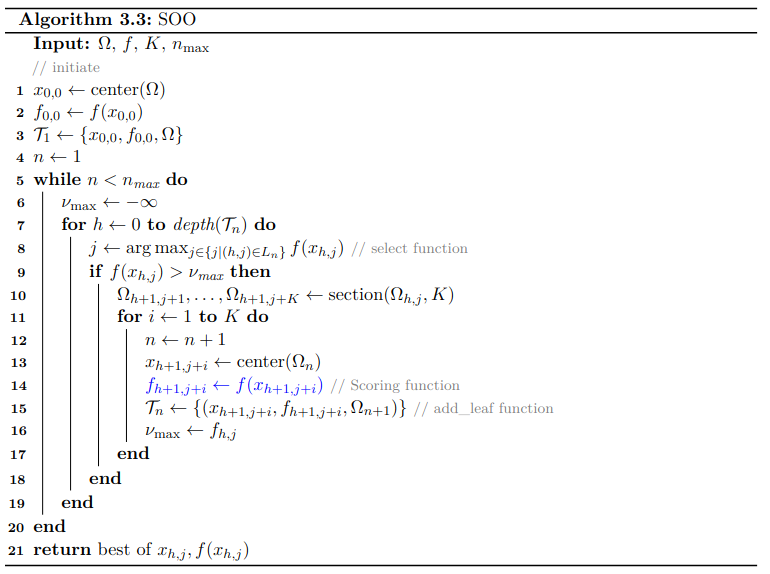
\includegraphics[trim={0 0 7cm 0},clip,height = 6.5cm]{imgs/algo/soo.png}
                \caption{SOO Algorithm}
            \end{figure}
        \end{column}
    \end{columns}

    \framebreak

    \begin{columns}
        \begin{column}{0.3\textwidth}
            \textbf{Surrogate Model Based Optimization : Bayesian Optimization with Gaussian Process (BO-GP)}

            Use Gaussian Process as a surrogate for the objective function, and optimize it to found the most promising point to evaluate
            
        \end{column}        
        \begin{column}{0.7\textwidth}
            \begin{figure}[h]
                \centering
                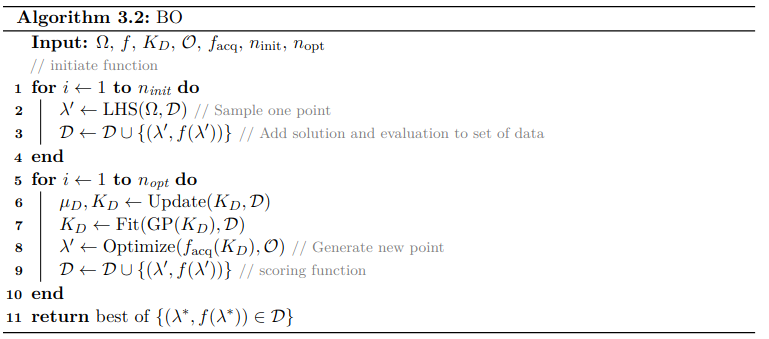
\includegraphics[height = 6cm]{imgs/algo/bo.png}
            \end{figure}
        \end{column}
    \end{columns}

    \framebreak

    \begin{columns}
        \begin{column}{0.5\textwidth}
            \textbf{Hybridation : Bayesian Multi-Scale Optimistic Optimization(BaMSOO)}

            Replace the scoring of SOO with a BO-GP based approximation to determine if it's relevant to evaluate the point.
            \begin{equation}
                \begin{split}
                \mathcal{UCB}(x| \mathcal D_t) = \mu(x|\mathcal D_t) +  B_N * \sigma(x|\mathcal D_t) 
                \\ \text{with } B_N = \sqrt{2 \log (\pi^2 N^2/6 \eta)} , \eta \in (0,1)      
                \end{split}  
                \label{eq:ucb}
            \end{equation}
            
        \end{column}        
        \begin{column}{0.5\textwidth}
            \begin{figure}[h]
                \centering
                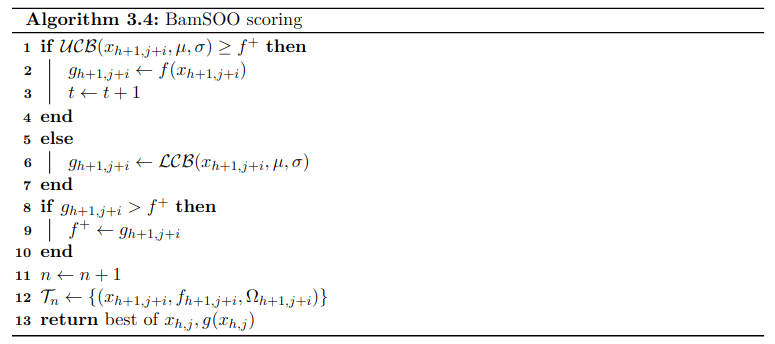
\includegraphics[trim={0 0 12cm 0},clip,height = 5cm]{imgs/algo/bamsoo_score.png}
            \end{figure}
        \end{column}
    \end{columns}

        
\end{frame}
%%%%%%%%%%%%%%%%%%%%%%%%%%%%%%%%%%%%%%%%%%%%%%%%%%%%%%%

%%%%%%%%%%%%%%%%%%%%%%%%%%%%%%%%%%%%%%%%%%%%%%%%%%%%%%%
\section{Experiments}
\frame{\sectionpage}
\begin{frame}{Experimental Setup}
    Experiments presented in this paper were carried out using the Grid'5000 testbed, supported by a scientific interest group hosted by Inria and including CNRS, RENATER and several Universities as well as other organizations (see https://www.grid5000.fr).\\


    One evaluation on chuc cluster, using 4*A100 40G of VRAM GPU, is taking around 40 minutes. Each algorithms have a budget of 50 evaluations, including the 10 sampling evaluation of BO. 
    
\end{frame}
%---------------------------------- Sampling experiment -------------------------------
\begin{frame}[allowframebreaks]{Sampling experiment : Latin Hypercube Sampling}
    
    \begin{columns}
        \begin{column}{0.45\textwidth}
        Objective : explore the search space and make a reference for other algorithms.
        \begin{block}{Analysis}
            \begin{itemize}
                \item Top scores : \\ \quad Hellaswag : 47.9\% \\ \quad MMLU : 37.6\%
                \item High range for Hellaswag, allowing to discriminate efficiently between solutions.
            \end{itemize}
            
        Running time : arround 36 hours
        
        \end{block}   
    \end{column}

    \begin{column}{0.45\textwidth}
        \begin{figure}
            \centering
            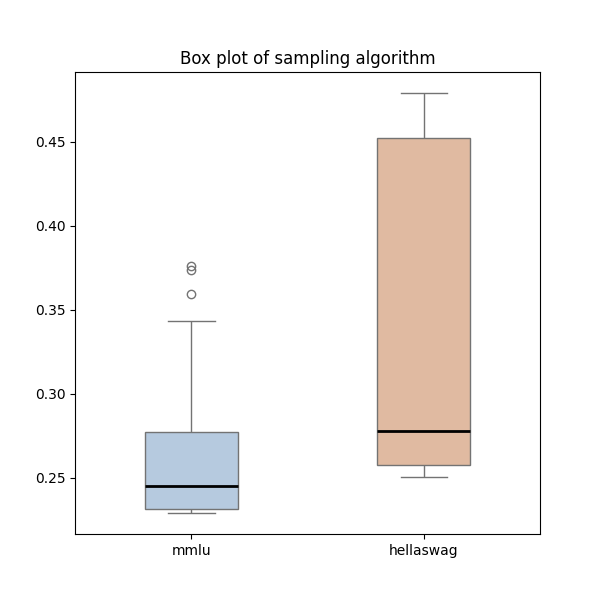
\includegraphics[width = \textwidth]{imgs/experiments/lhs_box_plot.png}     
            \caption{Distribution of score for sampling experiment}         
        \end{figure}
         
    \end{column}
\end{columns}  
    %%%%%%%%%%%%%%%%%%%%%%%%%%%%%%%%%%% BREAK %%%%%%%%%%%%%%%%%%%%%%%%%%%%%%%%%%%
    \framebreak

    \begin{columns}
        \begin{column}{0.3\textwidth}
        \begin{figure}
            \centering
            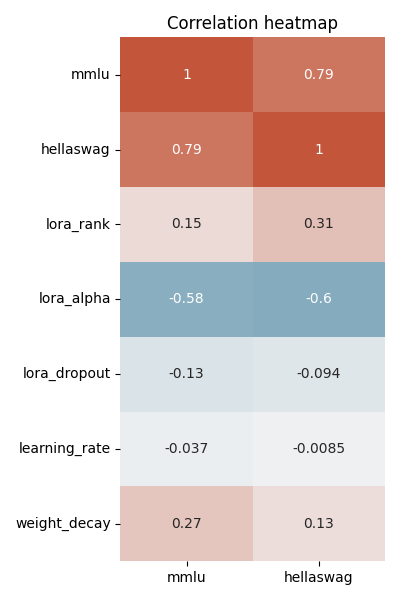
\includegraphics[width = \textwidth]{imgs/experiments/lhs_correlation.png}     
            \caption{Correlation between variables and metrics}         
        \end{figure}
         
        \end{column}
        \begin{column}{0.6\textwidth}
            \begin{block}{Correlation between metrics}
                With 79\% of correlation, Hellaswag and MMLU accuracy are relevant as validation/testing metrics.
            \end{block}
            \begin{block}{Correlation between variables and metrics}
                High factor variables : LoRA alpha the Lora rank / weight decay.\\
                TO DO : verify with other experiment the relevance of using dropout and learning rate.
            \end{block}
        \end{column}
    \end{columns}

\end{frame}



%---------------------------------- Bayesian Optimization -------------------------------
\begin{frame}[allowframebreaks]{BO (waiting for results)}
    
    \begin{columns}
    
        \begin{column}{0.6\textwidth}
            \begin{block}{Score evolution}
                \begin{figure}
                    \centering
                    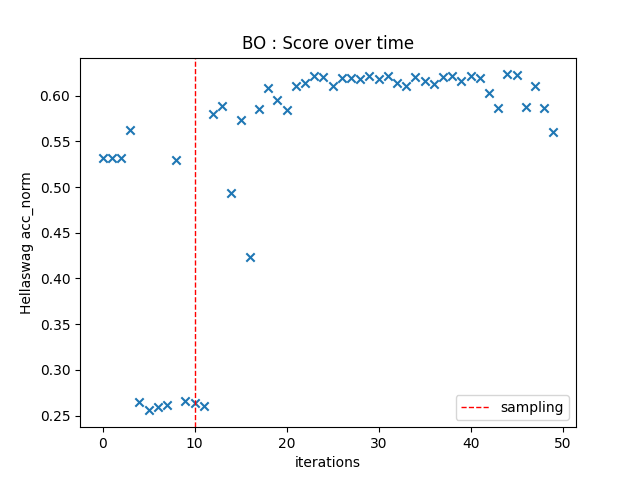
\includegraphics[width = 7.5cm]{imgs/plots/exp12_score_over_time.png}
                    \caption{Score over time}
                \end{figure}
            
            \end{block}   
        \end{column}

        \begin{column}{0.4\textwidth}
            \begin{block}{Results}
                Best score : 62.3\%, achieved after X iterations. \\   
                Wait for MMLU to look at overfitting            
            \end{block}

            \begin{block}{Behavior}
                \begin{itemize}
                    \item 0 -> 10 : sampling (LHS)
                    \item 10 -> 25 : converge to high score
                    \item 25 -> 40 : high score
                    \item 40 -> 50 : search unexplored space
                \end{itemize}
                
            \end{block}
             
        \end{column}
    \end{columns}    

    %%%%%%%%%%%%%%%%%%%%%%%%%%%%%%%%%%% BREAK %%%%%%%%%%%%%%%%%%%%%%%%%%%%%%%%%%%
    \framebreak

    \begin{columns}
    
        \begin{column}{0.65\textwidth}
            \begin{block}{Exploitation of the search space}
                rank, alpha and learning rate seem to converge fast\\
                weight decay converge slowly to the top during high score phase\\
                
                dropout does not converge, linked with weak correlation to metrics => relevant Hyperparameter ?? 
            \end{block}
        \end{column}

        \begin{column}{0.35\textwidth}
            \begin{figure}
                \centering
                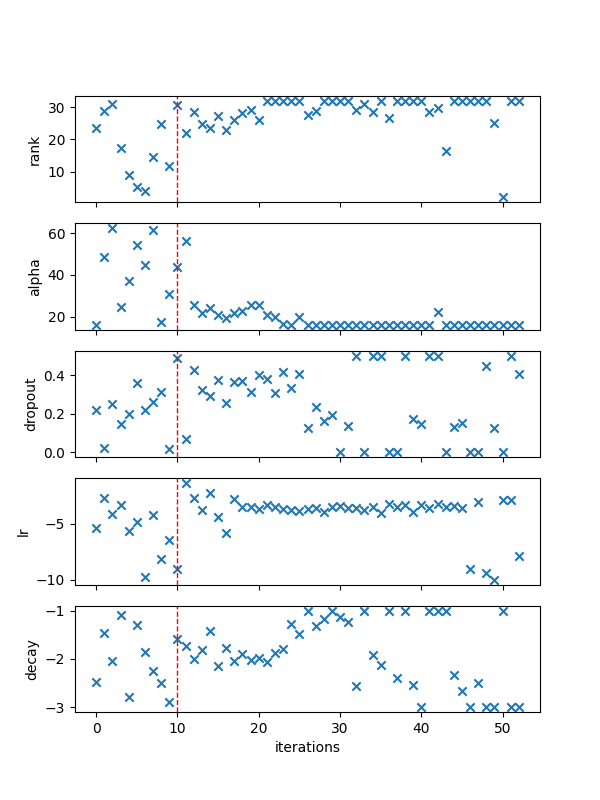
\includegraphics[width = \textwidth]{imgs/plots/exp12_variables_over_time.png}
                \caption{Variables over time}
            \end{figure}
            
            
        \end{column}
    \end{columns}  
\end{frame}

%---------------------------------- Optimization -------------------------------
\begin{frame}[allowframebreaks]{SOO(waiting for results)}
    
    \begin{columns}
    
        \begin{column}[t]{0.6\textwidth}
            \begin{block}{Score evolution}
                
                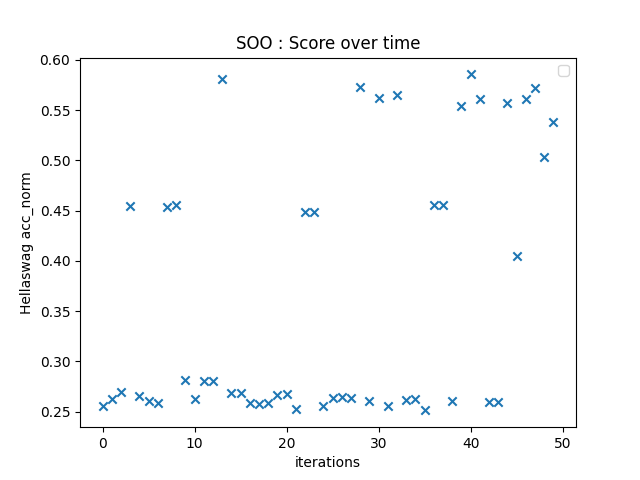
\includegraphics[width = 7.5cm]{imgs/plots/exp10_score_over_time.png}
            
            \end{block}   
        \end{column}

        \begin{column}[t]{0.4\textwidth}
            \begin{block}{Results}
                Best score : 58.4\%\\              
            \end{block}

            \begin{block}{Behavior}
                Slow convergence, need more than 50 iterations to converge to more depth. 
                Max depth : 6
                A lot of unpromising point to explore
                
            \end{block}
            
            
        \end{column}
    \end{columns}   
    
    \framebreak

    \begin{columns}
    
        \begin{column}{0.65\textwidth}
            \textbf{Score by variables and Varibles over iterations}
                \begin{figure}[h]
                    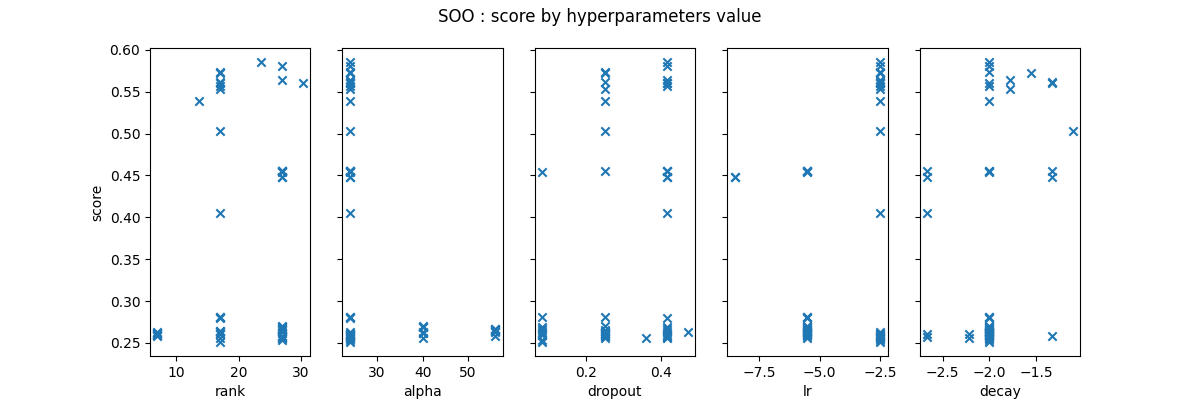
\includegraphics[width = \textwidth]{imgs/plots/exp10_score_by_hp.png}
                \end{figure}     
        \end{column}

        \begin{column}{0.4\textwidth}
            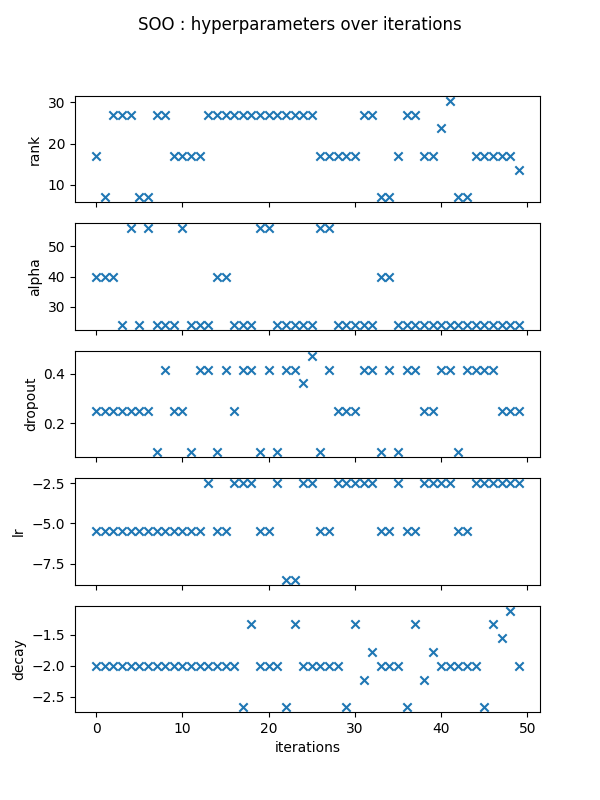
\includegraphics[height = 7cm]{imgs/plots/exp10_variables_over_time.png}
            
            
        \end{column}
    \end{columns}  
\end{frame}

%---------------------------------- Optimization -------------------------------
\begin{frame}[allowframebreaks]{BaMSOO}
    
    \begin{columns}
    
        \begin{column}[t]{0.6\textwidth}
            \begin{block}{Score evolution}
                
                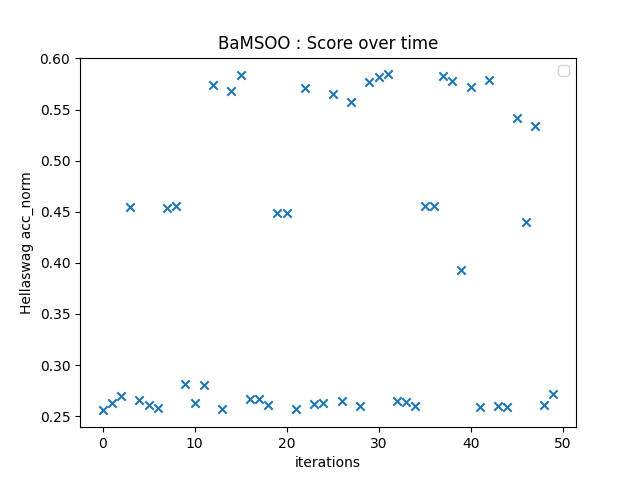
\includegraphics[width = 7.5cm]{imgs/plots/exp11_score_over_time.png}
            
            \end{block}   
        \end{column}

        \begin{column}[t]{0.4\textwidth}
            \begin{block}{Results}
                Best score : 58.5\%\\
                Not so much approximations, need to increase $\eta $ in equation \ref{eq:ucb} to speed the convergence              
            \end{block}
            
            
        \end{column}
    \end{columns}    

    \framebreak

    \begin{columns}
    
        \begin{column}{0.65\textwidth}
            \textbf{Score by variables and Varibles over iterations}
                \begin{figure}[h]
                    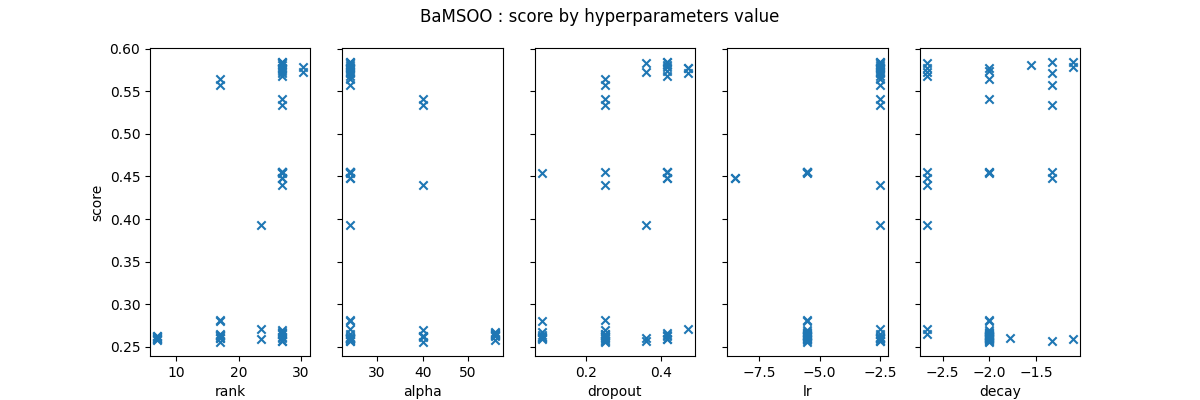
\includegraphics[width = \textwidth]{imgs/plots/exp11_score_by_hp.png}
                \end{figure}     
        \end{column}

        \begin{column}{0.4\textwidth}
            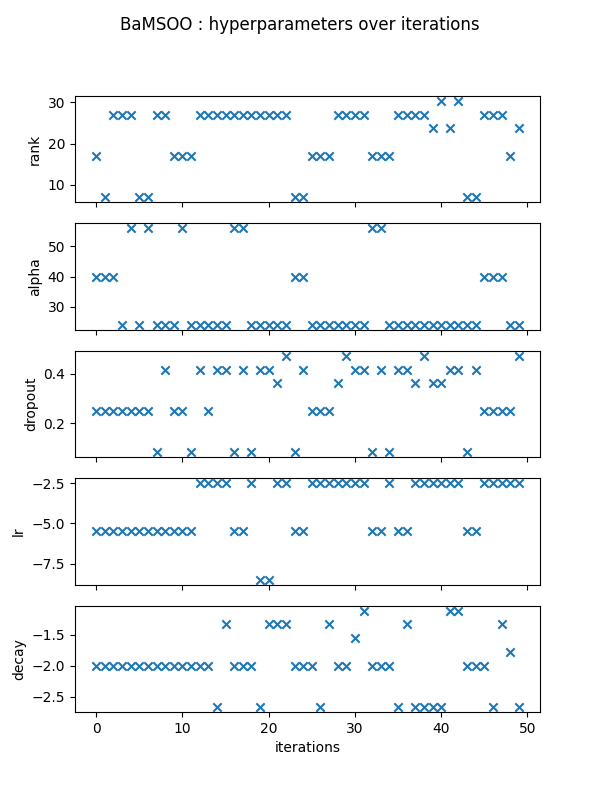
\includegraphics[height = 7cm]{imgs/plots/exp11_variables_over_time.png}
            
            
        \end{column}
    \end{columns}  
\end{frame}

%%%%%%%%%%%%%%% COMPARISON %%%%%%%%%%%%%%
\begin{frame}{Comparison (waiting results)}

    \begin{table}[ht!]
        \centering
        \begin{tabular}{|c||c|c||c|c|c|}
        \hline
           Datasets  & Lower (LHS) & Upper & BO & SOO & BaMSOO \\
        \hline
           Hellaswag  & 47.9 & 69.8* & X & X & X \\
           MMLU & 37.6 & 49.3 & X & X & X  \\
        \hline
        \end{tabular}
        \caption{Bounds on accuracy for validation and testing dataset}
        \label{tab:bounds}
    \end{table}

\end{frame}
%%%%%%%%%%%%%%%%%%%%%%%%%%%%%%%%%%%%%%%%%%%%%%%%%%%%%%%


\section{Conclusion}
\begin{frame}{Conclusion}

\begin{block}{review}
    On a sequential comparaison, BO-GP algorithms is the most efficient between theses 3 algorithms, even considering the exploitation made by BamSOO algorithms. But this kind of performance needs to efficiently scale to be able to be usable with very expensive function, especially if the evaluation can't be distributed. 

    With it's acceleration using GP, BaMSOO keep most of the SOO abilities, in particular it's parallelism inate abilities, but achieve to be efficient with a smaller number of evaluation. 

    To be able to effectively compare theses approaches, it's necessary to look at higher dimensionnal problem. 
    
\end{block}

\begin{block}{Perspective}
    \begin{itemize}
        \item Expand search space : add dimensions (Adam momentum, precision, matrices to apply LoRA)
        \item use more training datasets
        \item make a distributed implementation
    \end{itemize}
    
\end{block}


\end{frame}

\
\begin{frame}[allowframebreaks]{Bibliography}
\printbibliography[]
\nocite{*}
\end{frame}






%%%%%%%%%%%%%%%%%%%%%%%%%%%%%%%%%%%%%%%%%%%%%%%%%%%%%%%

%% Le texte est modifiable en changeant \thankyou
\renewcommand{\thankyou}{Thank You.}
\frame{\merci}

%%%%%%%%%%%%%%%%%%%%%%%%%%%%%%%%%%%%%%%%%%%%%%%%%%%%%%% 

\end{document}

%%%%%%%%%%%%%%%%%%%%%%%%%%%%%%%%%%%%%%%%%%%%%%%%%%%%%%%
%%
%%%%%%%%%%%%%%%%%%%%%%%%%%%%%%%%%%%%%%%%%%%%%%%%%%%%%%%

